\section{Causality}
\begin{itemize}
	\item Causality is about testing whether one event (\textit{effect}) is the result of the occurrence of another event (\textit{cause}), i.e. a change in the cause will lead to a change in the effect. It differs from correlation by \textit{explaining}/\textit{finding} the relationship behind variables
	\item While we look at the data distribution for correlation, we are focusing on the generation mechanism of the data in causality. While in statistics we then like to predict the next observation (or its likelihood), causality is interested in what happens if we perform interventions (setting a variable to a certain value)
	\item The most important operator in causality is the \textbf{do-operator}: $p(A=a|\Cdo(B=b))$. It differs from the standard conditional probability as follows by not assuming that we have observed $B=b$, but that we externally set the value of $B$. This means that we cannot infer anything from its parents as in standard conditionals (if we observe $B=b$, then this usually gives us information about its parents).
	
	Note that there are cases where $p(A=a|\Cdo(B=b))=p(A=a|B=b)$. One obvious example for this is when $B$ has no parents in its corresponding graphical model.
	\item We start with a discussion about the terminology in causality, and then take a closer look at Causal Bayesian networks and causal reasoning
\end{itemize}
\subsection{Causality terminology}
\begin{itemize}
	\item $A$ is said to \underline{cause} $B$ if changing $A$ leads to a change in $B$
	\item Similar to graphical models, we can define Causal graphs that represent causal relationships. An edge from $A$ to $B$ in the graph means that $A$ \textit{causes} $B$ even if all other variables are kept fixed. Figure~\ref{fig:causality_overview_causal_graphs} gives an overview.
	
	\begin{figure}[ht!]
		\centering
		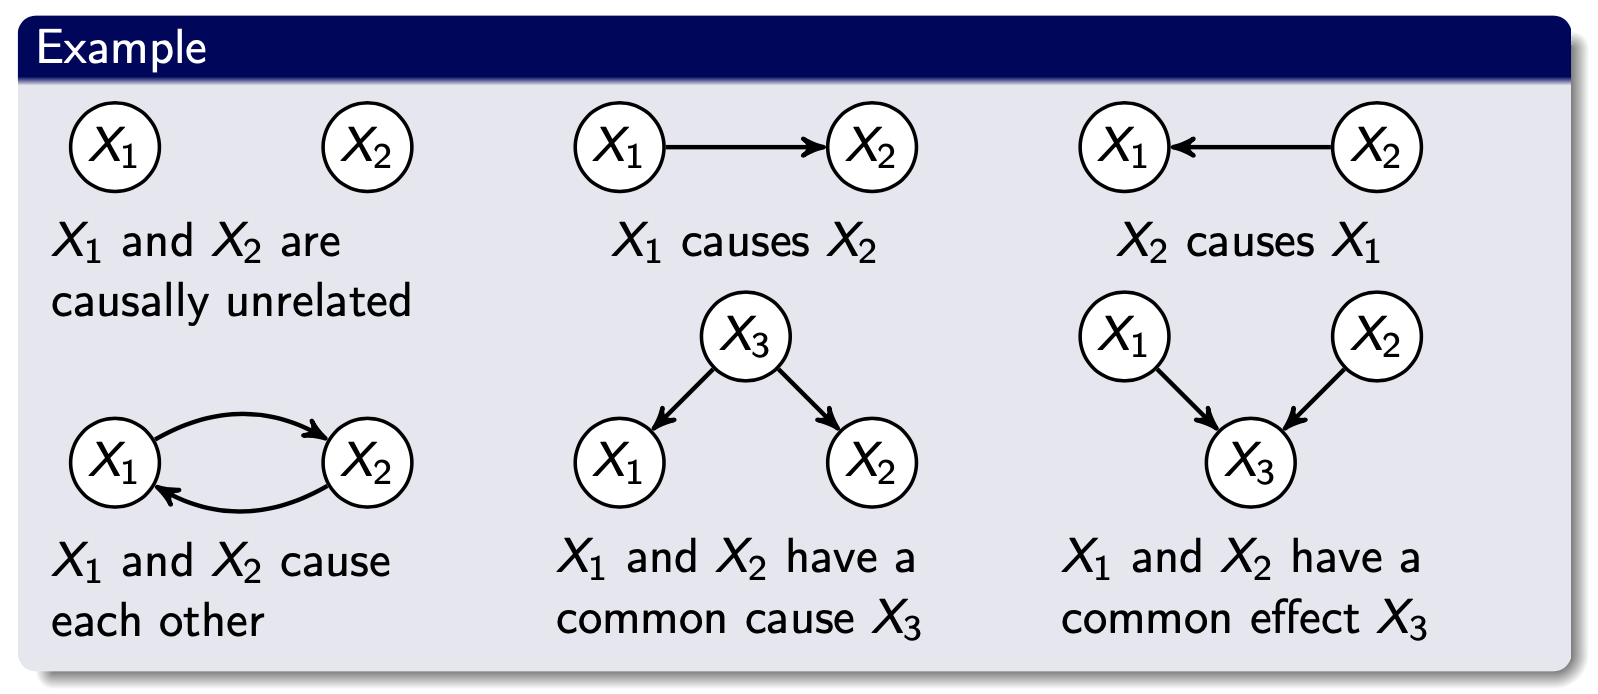
\includegraphics[width=0.6\textwidth]{figures/causality_overview_causal_graphs.png}
		\caption{Examples of causal graphs (retrieved from lecture notes).}
		\label{fig:causality_overview_causal_graphs}
	\end{figure}
	
	Note that these graphs can contain loops, which represents a feedback loop (a change in $A$ leads to a change in $B$, and a change in $B$ leads to a change in $A$). However, we will not take a closer look at those.
	
	\item We can interpreted node relationships in the graph as causal relations:
	\begin{itemize}
		\item $A$ is a \textit{parent} of $B$ $\implies$ $A$ is a direct cause of $B$
		\item $A$ is a \textit{child} of $B$ $\implies$ $A$ is a direct effect of $B$
		\item $A$ is a \textit{ancestor} of $B$ (e.g. $A\to C \to B$) $\implies$ $A$ is a cause of $B$. Note that if we fix $C$, there is no effect of $A$ on $B$. Hence, there is no direct edge.
		\item $A$ is a \textit{descendant} of $B$ (e.g. $B\to C\to A$) $\implies$ $A$ is an effect of $B$.
	\end{itemize}
	\item We use the notation $\mathcal{G}_{\overline{X}}$ to denote a sub-graph of $\mathcal{G}$ in which the incomming edges of $X$ are removed. This is useful for discussing when $X$ is set externally (hence, no influence of parents of $X$ in that case).
	
	Similarly, $\mathcal{G}_{\underline{X}}$ is $\mathcal{G}$ without the outgoing edges of $X$.
	\item  A \textbf{perfect intervention} $\Cdo(X=\xi)$ means that we force $X$ to eb the value $\xi$. Thereby, the graph $\mathcal{G}$ changes to $\mathcal{G}_{\overline{X}}$
	\begin{itemize}
		\item To perform intervention, we require \textit{modularity}, meaning that we can manipulate $X$ without influencing any other variables in the graph $\bm{V}\setminus X$
		\item This can be a challenge in real systems, but in our theoretical models, we can assume that we are able to do so
	\end{itemize}
	\item A variable $H$ is a \textbf{confounder} of $X$ and $Y$ (i.e. $H$ confounds $X$ and $Y$) if there is a directed path from $H$ to $X$ which does not include $Y$, and same from $H$ to $Y$. Note that it is still allowed to have other paths between $X$ and $Y$. Examples of confounders are shown in Figure~\ref{fig:causality_confounders_examples}.
	
	\begin{figure}[ht!]
		\centering
		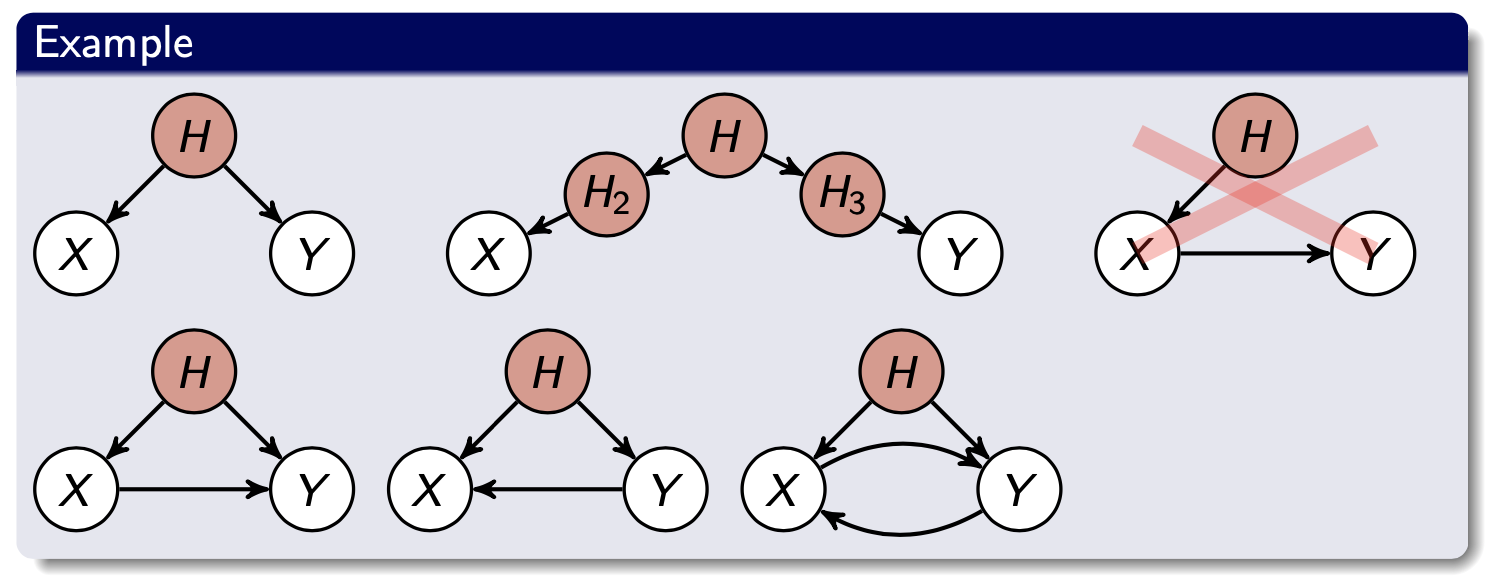
\includegraphics[width=0.5\textwidth]{figures/causality_confounders_examples.png}
		\caption{Examples of when a node $H$ is a confounder of $X$ and $Y$ (retrieved from lecture notes).}
		\label{fig:causality_confounders_examples}
	\end{figure}

	\item \textbf{Reichenbach's principle} sets correlation and causality into relation: if $X$ and $Y$ are correlated/depending on each other, then there is either a causal relation of the type $X\to Y$, $Y\to X$ or there exists a confounder $H$ of $X$ and $Y$.
	\begin{itemize}
		\item Note that this principle can fail is we have a selection bias, meaning that the dataset of $X$ and $Y$ was obtained by only including samples that are conditional on some (possibly latent) event.
	\end{itemize}
\end{itemize}

\subsection{Causal Bayesian Networks}
\begin{itemize}
	\item An subspace of causal networks with many assumptions/limitations, but therefore easier to work with, are Causal Bayesian Networks. We make the following assumptions:
	\begin{itemize}
		\item No confounding % A graph $\mathcal{G}$ does not contain any confounder
		\item A graph $\mathcal{G}$ does not contain any loops
		\item We do not have any selection bias in the data, nor measurements error or time dependencies
	\end{itemize}
	\item We call a Bayesian Network causal if:
	\begin{itemize}
		\item Directed edges correspond with directed causal relations
		\item After a perfect intervention $\Cdo(X_{I}=x_I)$, the probability density becomes:
		\begin{equation*}
		\tcbox[nobeforeafter]{\(
			\begin{split}
				p\left(\bm{X}_{\bm{V}\setminus I}|\Cdo(X_I=x_I)\right) = \prod_{i\in \bm{V}\setminus I} p\left(x_i|\bm{x}_{\text{pa}_i}\right)
			\end{split}
			\)}
		\end{equation*}
		
	\end{itemize}
\end{itemize}

\subsection{Causal Reasoning}
\begin{itemize}
	\item The goal of causal reasoning is to estimate $p(y|\Cdo(X=x))$. If we can express it in terms of the observational distribution $p(x,y,...)$ we say it is \textbf{identifiable} from the observational distribution. 
	
	Note that it does not necessarily require all variables to be observable.
	\item Assume we have the following Bayesian Causal Network:
	
	\begin{figure}[ht!]
		\centering
		\tikz{ %
			\node[latent] (X) {$X$} ; %
			\node[latent, right=of X] (H) {$H$} ; %
			\node[latent, below=of H] (Y) {$Y$} ; %
			
			\edge{H}{X};
			\edge{H}{Y};
			\edge{X}{Y};
		}
	\end{figure}

	The standard conditional distribution is:
	$$p(y|x)=\int p(y|h,x)p(h|x)dh$$

	Now, assume we perform a perfect intervention on $X$, i.e. $\Cdo(X=x)$. What happens is that we neglect the effect of $H$ on $X$, \textit{but} we still need to consider the effect of $H$ on $Y$. Hence, the conditional becomes:
	$$p(y|\Cdo(X=x))=\int p(h)p(y|h,x)dh$$
	The important thing is that we have to prevent that changing $X$ influences $H$ by ``back-reasoning'' (i.e. $H$ causes $X$, but observing $X$ gives us information of $H$), which again influence $Y$. This is because we cannot change $H$ by just forcing $X$ to a value, as we \textit{overwrite} the effect of $H$ on $X$. Hence, we have to explicitly remove its dependency on $X$ in the integral.
	
	%The result indicates that we had to \textit{adjust} the conditional probability for the effect of $H$. But suppose, we would not have the connection between $H$ and $Y$. Then, we would not have to adjust for $H$, and get $p(y|\Cdo(X=x))=p(y|x)$.
	\item We can derive a more general algorithm for deciding, for which variables we need to \textit{adjust} our conditional probability for. This can be done in a very similar manner to d-separation, as we need to find all variables, that are implicitly changed by setting $X$ to a certain value (i.e. variables that influence the decision of which value $X$ can have), but then also influence $Y$. We do not want this influence because by forcing $X$ to be a certain value, we cannot change variables that cause $X$. Hence, we are trying to find a set of variables $S$ which break these kind of influences, and remove their dependency with $X$.
	
	\item In general, we can determine whether $S$ is a sufficient set of variables we are adjusting by the following check:
	
	\begin{tcolorbox}[colback=white!80!gray,colframe=gray!75!black,title=Back-door criterion]
		A set of variables $S$ satisfies the back-door criterion relative to a variable pair ($X$, $Y$), if:
		\begin{enumerate}
			\item $X, Y\not\in S$
			\item No node of $S$ is a descendant (i.e. child of a child etc.) of $X$
			\item $S$ blocks all paths from $Y$ to $X$ where we have an incoming edge to $X$ (other directions irrelevant for path itself). A path is blocked by $S$ if:
			\begin{enumerate}
				\item It contains a collider $...\rightarrow u \leftarrow ...$ such that $u$ is not an ancestor of a node in $S$
				\item It contains a non-collider $...\rightarrow u$, $...\rightarrow u \rightarrow ...$, $...\leftarrow u \rightarrow ...$ such that $u$ is in $S$
			\end{enumerate}
		\end{enumerate}
		Then $S$ is admissible for adjustment to find the causal effect of $X$ on $Y$:
		$$p(y|\Cdo(X=x))=\int p(y|X=x,S=s)p(S=s)ds$$
		If $S=\emptyset$: $p(y|\Cdo(X=x))=p(y|X=x)$
	\end{tcolorbox}	

	To find the actual set $S$, we can simply perform the algorithm backwards. First, find all paths from $Y$ to $X$ with an incoming edge to $X$. Then, we start with $S=\emptyset$, and try to block all paths by adding variables to $S$. In case that all paths were blocked from the beginning on, or no paths exist, we can stop with $S=\emptyset$.
	
	\item \underline{Examples}: 
	\begin{itemize}
		\item Consider the examples in Figure~\ref{fig:causality_backdoor_example}. Note that we usually try to find the smallest set of admissible variables as this simplifies the integral we have to take.
		
		\begin{figure}[ht!]
			\centering
			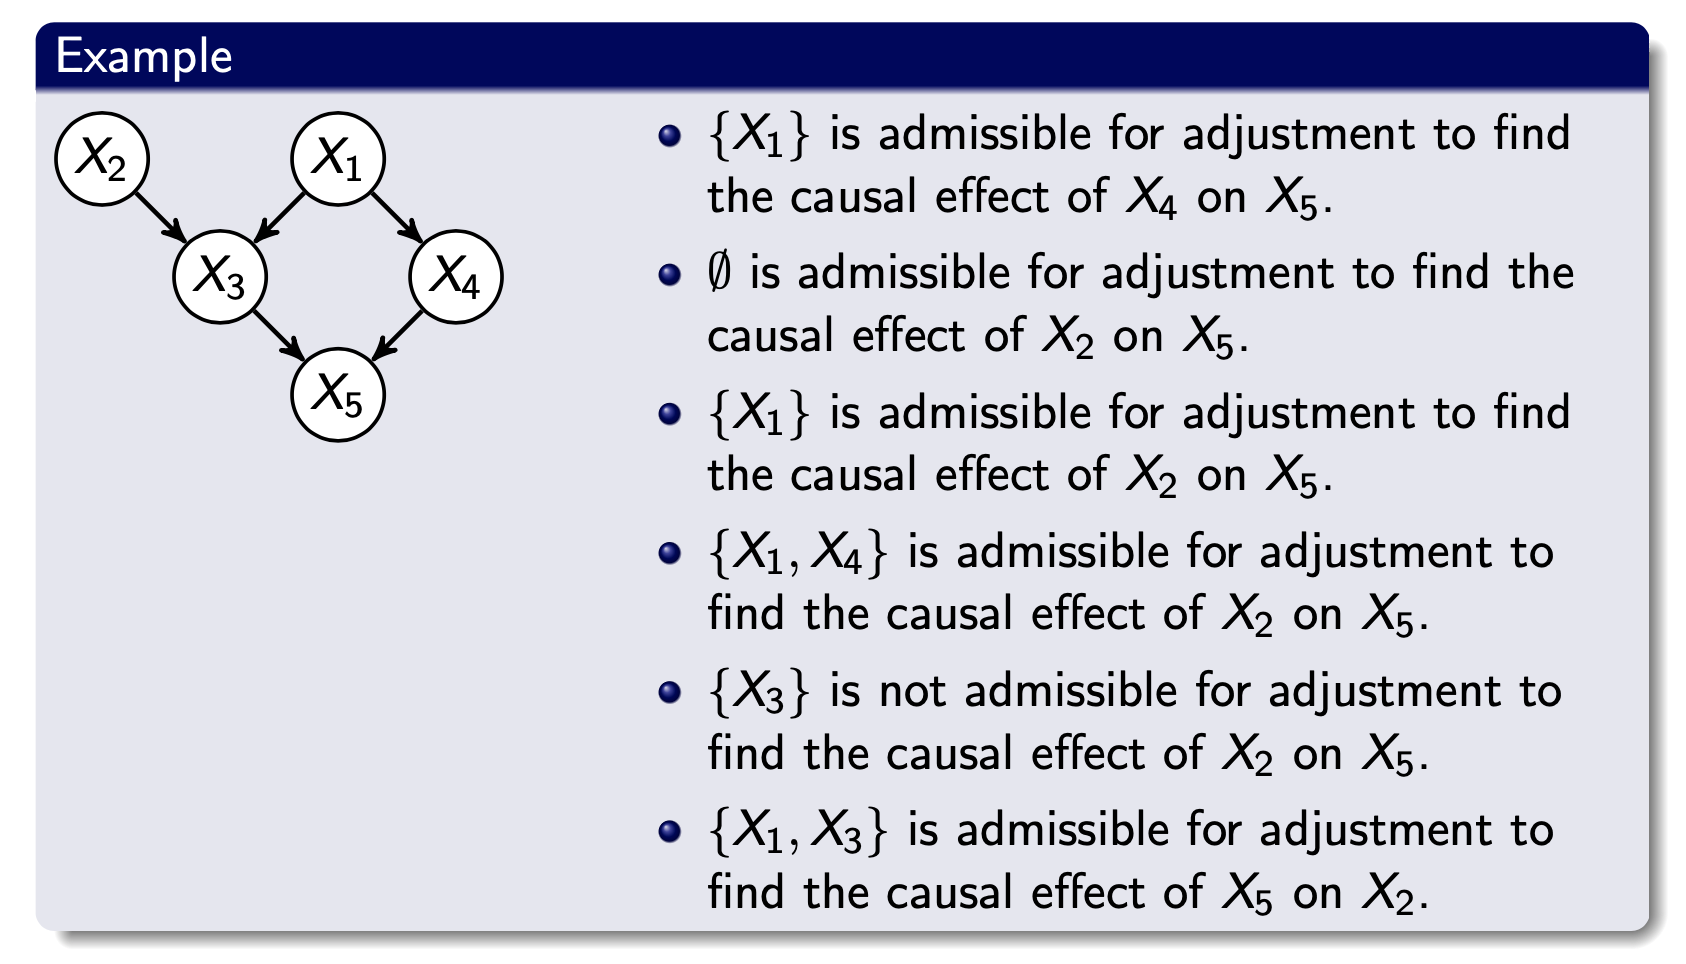
\includegraphics[width=0.5\textwidth]{figures/causality_backdoor_example.png}
			\caption{Example of admissible sets of variables for adjustment (retrieved from lecture notes).}
			\label{fig:causality_backdoor_example}
		\end{figure}
		\newpage
		\item Consider the following, slightly more complicated Causal Bayesian Network:
		\begin{figure}[ht!]
			\centering
			\tikz{ %
				\node[latent] (X1) {$X_1$} ; %
				\node[latent, below=of X1] (X3) {$X_3$} ; %
				\node[latent, right=of X3] (X4) {$X_4$} ; %
				\node[latent, right=of X4] (X5) {$X_5$} ; %
				\node[latent, above=of X5] (X2) {$X_2$} ; %
				\node[latent, below=of X3] (X7) {$X_7$} ; %
				\node[latent, right=of X7] (X6) {$X_6$} ; %
				\node[latent, right=of X6] (X8) {$X_8$} ; %
				
				\edge{X1}{X3};
				\edge{X1}{X4};
				\edge{X3}{X7};
				\edge{X4}{X7};
				\edge{X4}{X8};
				\edge{X7}{X6};
				\edge{X6}{X8};
				\edge{X5}{X8};
				\edge{X2}{X5};
				\edge{X2}{X4};
			}
		\end{figure}	
	
		We are trying to find the set $S$ admissible for adjustment for the causal effect of $X_7$ on $X_8$ (the two nodes on the bottom, left and right). We have to consider all paths with incoming edges to $X_7$, so from $X_3$ and $X_4$. To block the path $X_8\to X_4\to X_7$, we add $X_4$ to $S$: $S=\{X_4\}$. However, by doing this, we unblocked another path: $X_8\to X_5\to X_2\to X_4\to X_1\to X_3\to X_7$. $X_4$ is not longer a collider anymore, as it is included in $S$. So, we can either add $X_3$, or $X_5$, or even $X_1$ or $X_2$ to block this path. For example, we can take $S=\{X_3,X_4\}$, which is then admissible for adjustment as all paths are blocked.
	\end{itemize}
	\item Although we found a way to estimate what happens when we perform an intervention, the best way to find causal relations is to use randomized controlled trials. In a drug test, this would mean that we completely random assign a person to take the drug or not, ensuring that no underlying selection bias is in the process. By that, we should break all back-door paths (as there is nothing besides a coin flip that causes the event of  "taking the drug")

\end{itemize}